\section{Hardware}

There are two parts to this project; the algorithmic side of things, and the hardware on which this algorithm runs.
Here the details about the design and production of the PCB will be discussed, and explanations of why certain decisions were made.

\subsection{Schematic}
\label{sec:imple:hard:sch}
Before producing the PCB design the system was designed in gEDA Schematic software.
In order to keep the design easy to maintain a hierarchy was used, and the system split into multiple sections.
These sections are discussed below.

\begin{figure}[H]
	\centering
	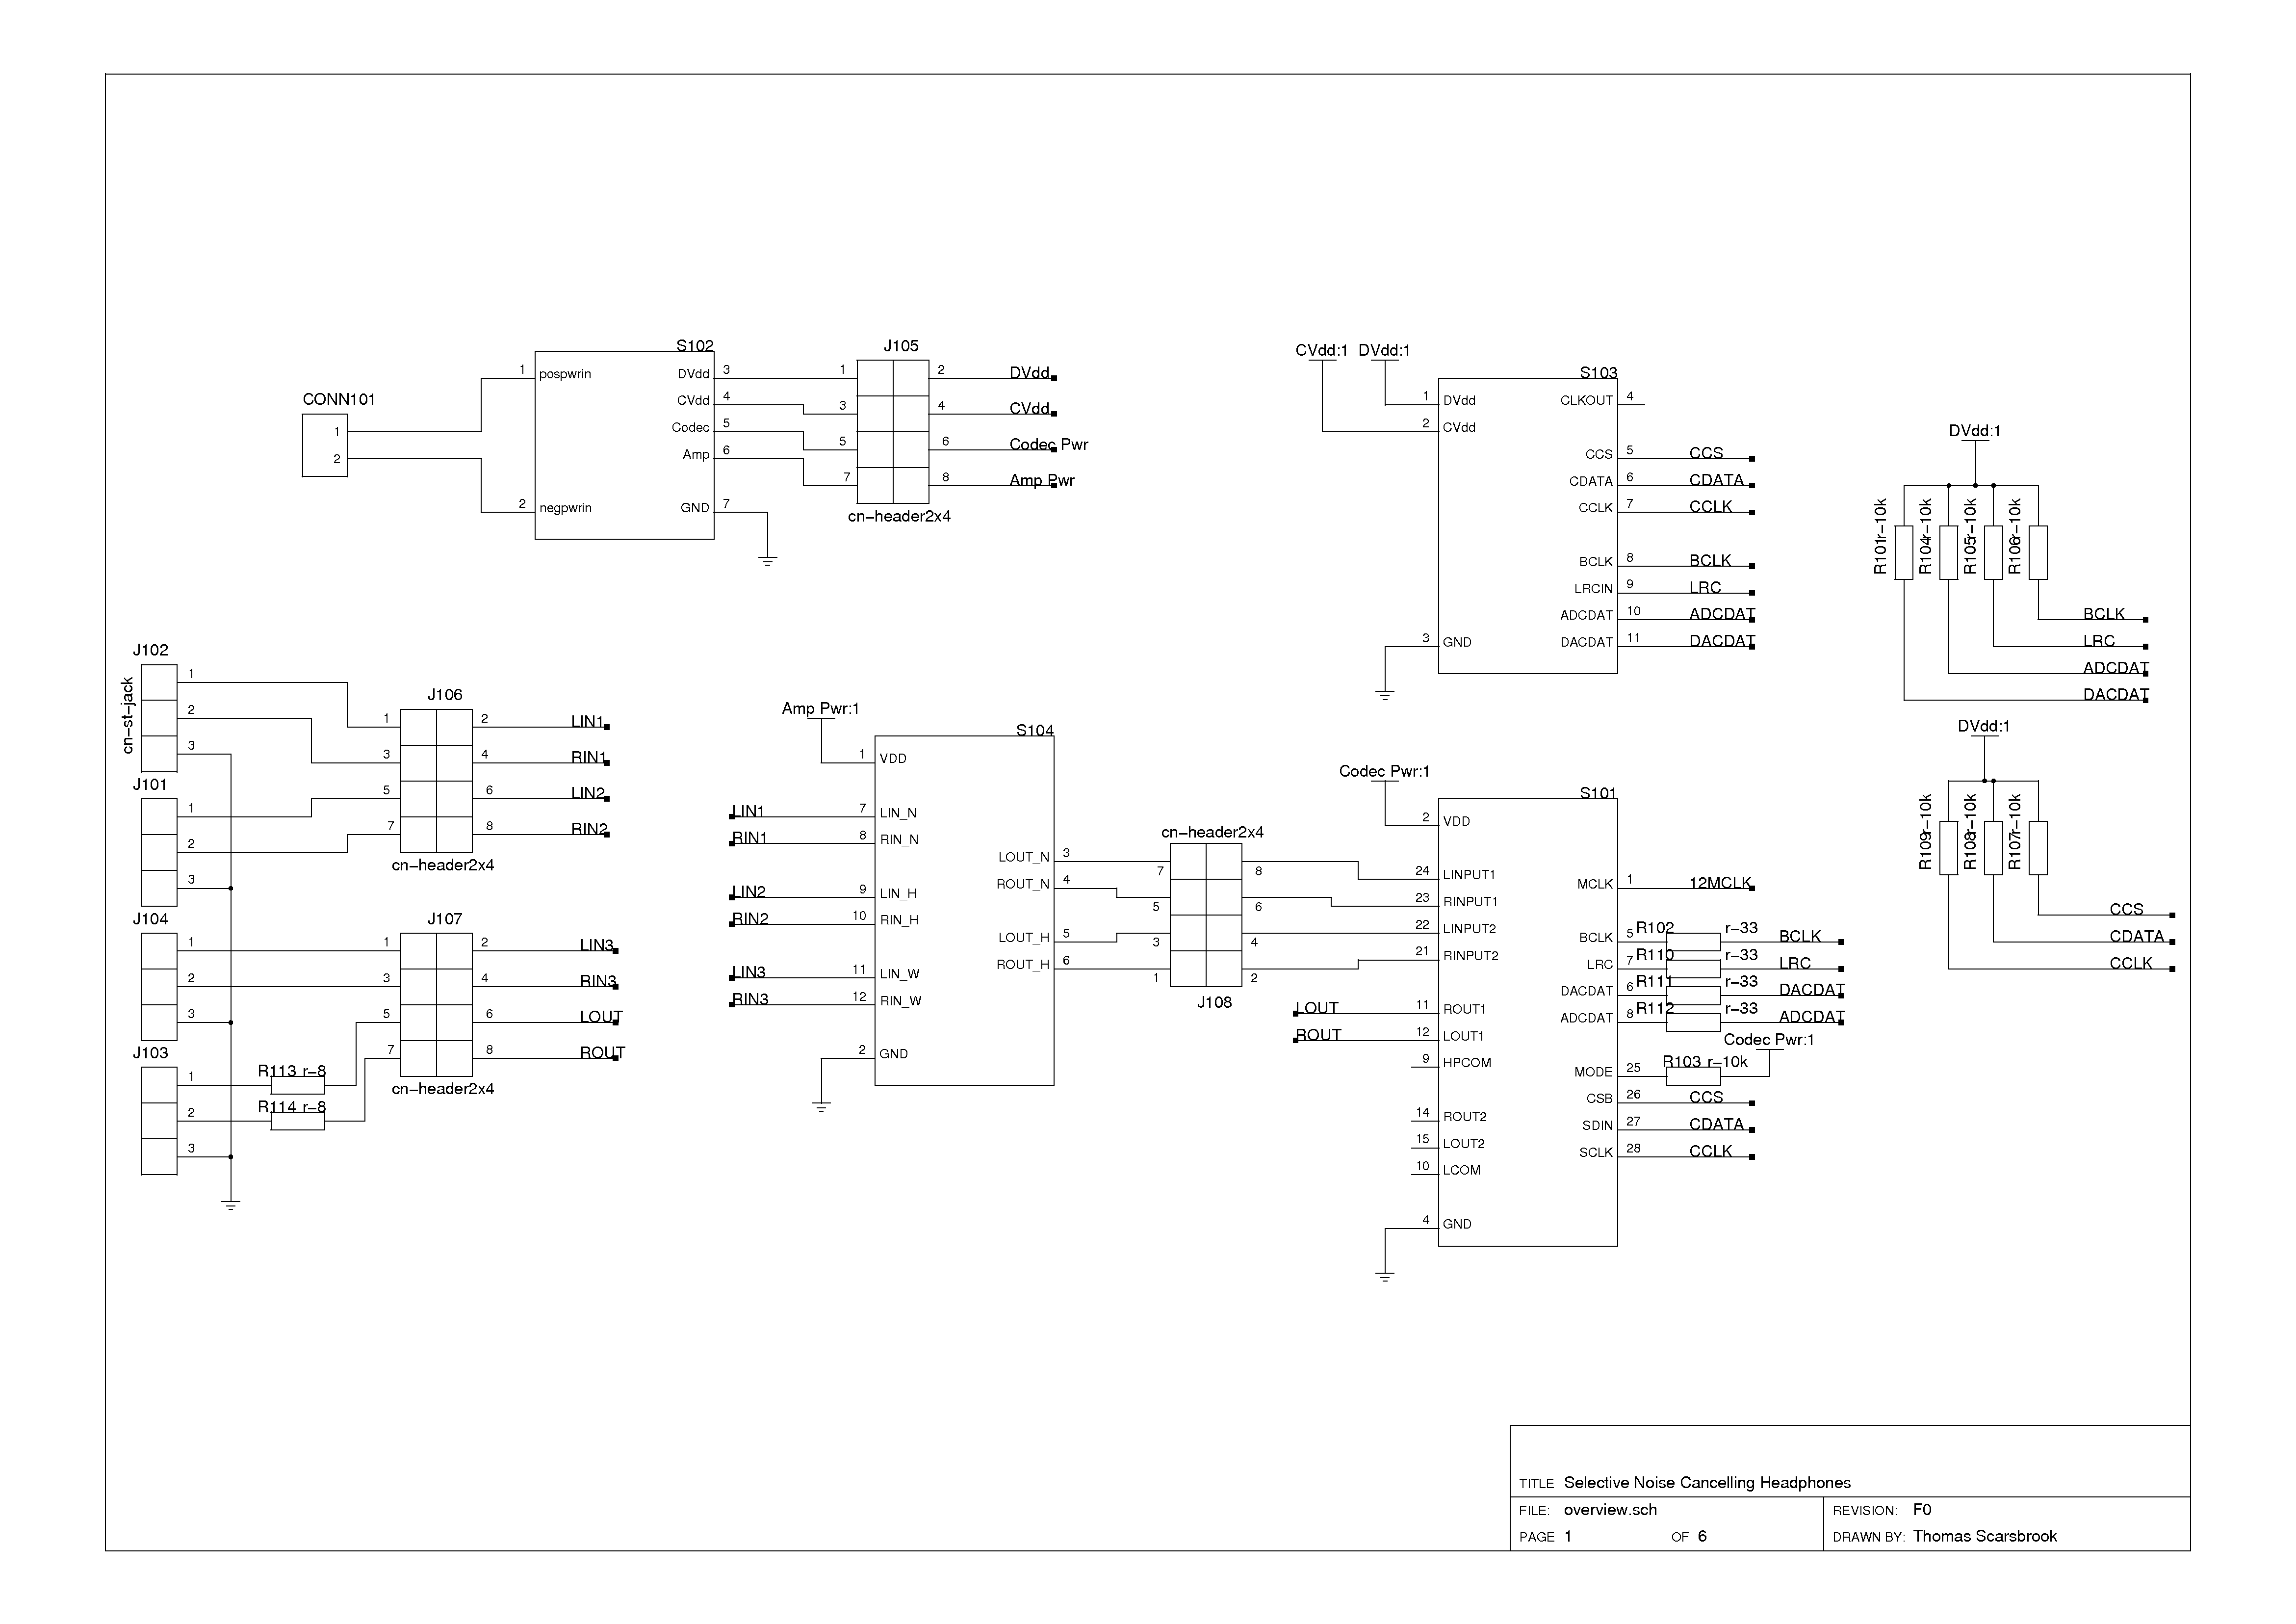
\includegraphics[width=\textwidth]{./img/overview.png}
	\caption{The top level schematic}
	\label{fig:overviewsch}
\end{figure}

\subsubsection{DSP}
At the heart of the project is the Digital Signal Processor.
This is the part that achieves all the calculations required by the cancelling algorithm.
The DSP chosen for this project was the Texas Instruments TMS320C6713B.
It was chosen as it had the desired interfaces required for communication with the codec, and was powerful enough to support the desired algorithms.
Another important factor used in the decision was that a development board for this DSP could be acquired, allowing the testing of code without requiring the PCB being produced.
Due to the complexity of the design, the DSP required two separate voltage levels, one for the core logic and one for the I/O.
Connectivity was required to them at multiple points around the device.
A significant number of decoupling capacitors were required at these power connections, in order to prevent noise from disrupting correct operation.
These capacitors can be seen in figure \ref{fig:dspdecouplingcaps}.

\begin{figure}[H]
	\centering
	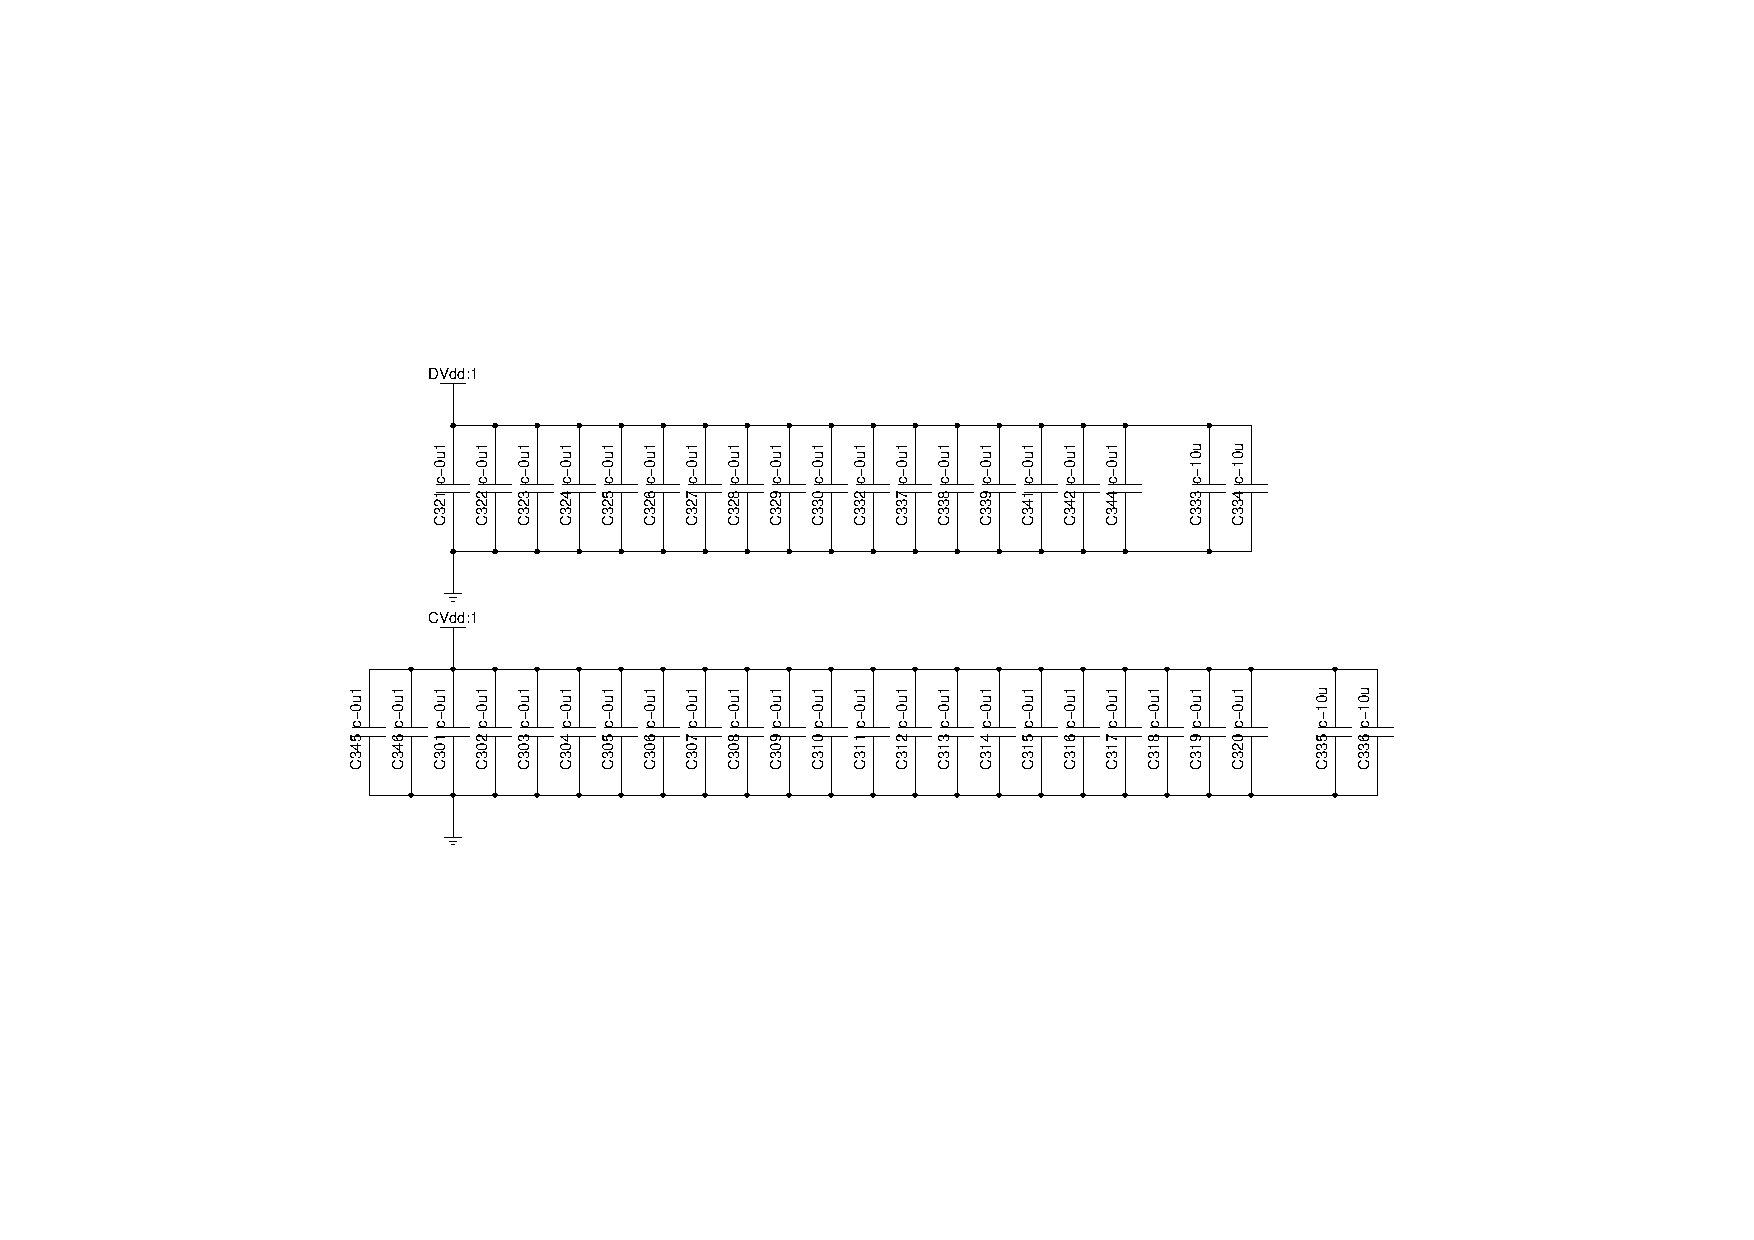
\includegraphics[width=\textwidth]{./img/dsp_decoupling.pdf}
	\caption{Decoupling capacitors for the DSP}
	\label{fig:dspdecouplingcaps}
\end{figure}

\noindent It is rather difficult to tell how code is operating on a DSP, due to the fact that the internals cannot be probed.
This becomes harder when debugging, as the code could be causing the DSP to crash.
If this were to happen then it has the potential to cause any debugging software to crash also, preventing the use of a stack trace.
As a way to circumvent this issue, a couple of LEDs were added to the DSP, connected to the general purpose I/O pins.
These could then be used for debugging, and potentially to display details to the user in a final product.

\begin{figure}[H]
	\centering
	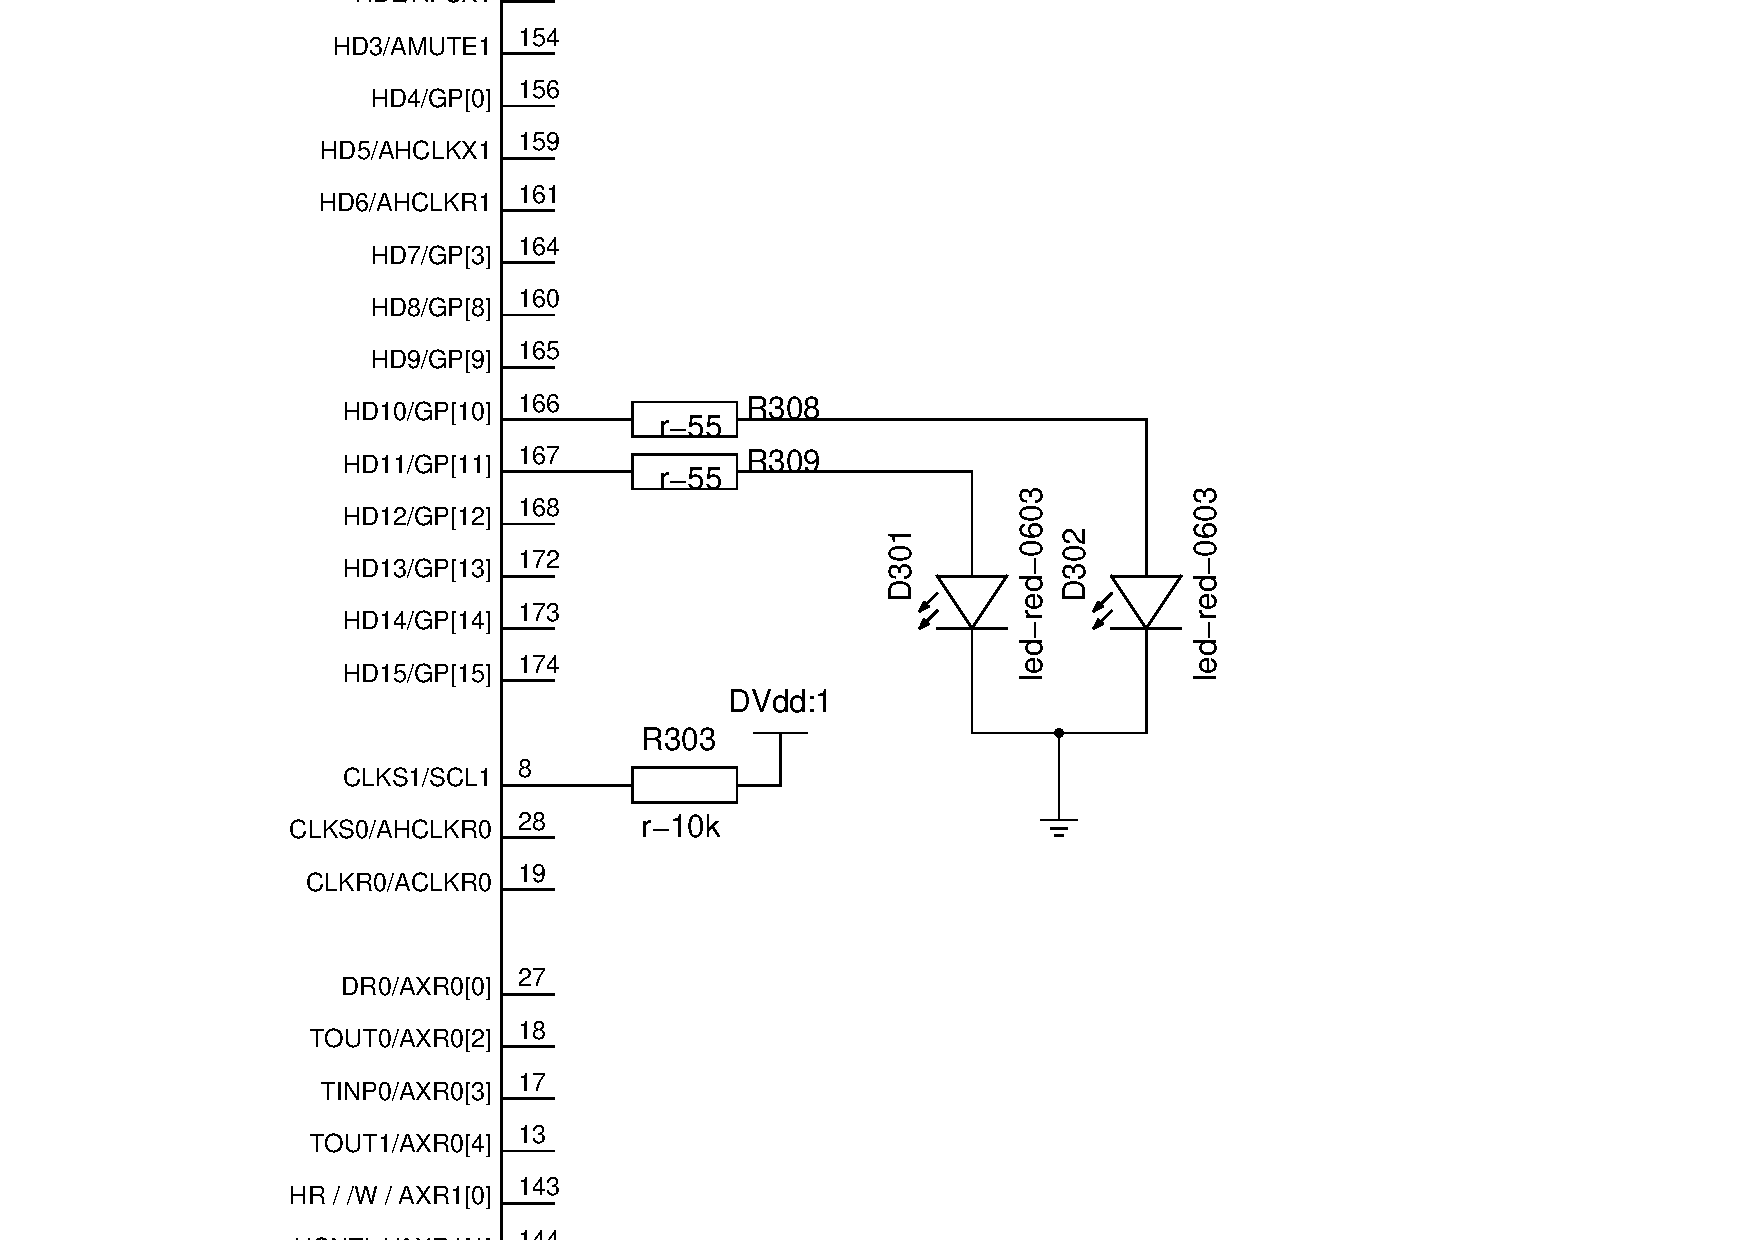
\includegraphics[width=\textwidth]{./img/dsp_LEDs.pdf}
	\caption{Debugging LEDs for the DSP}
	\label{fig:dspdebugleds}
\end{figure}

\noindent In order to program and debug the DSP, a JTAG header was set up.
The header used was compatible with the standard Texas Instruments 14 pin JTAG connector, to enable use of standard programming tools.
The pin layout for this header can be seen in table \ref{tab:jtagpinout}.

\begin{table}[H]
	\centering
	\begin{tabular}[c]{| c | l |}
		\hline
		Pin	& Function	\\
		\hline
		1	& TMS		\\
		2	& nTRST		\\
		3	& TDI		\\
		4	& GND		\\
		5	& $DV_{dd}$	\\
		6	& KEY		\\
		7	& TDO		\\
		8	& GND		\\
		9	& RTCK		\\
		10	& GND		\\
		11	& TCK		\\
		12	& GND		\\
		13	& EMU0		\\
		14	& EMU1		\\
		\hline
	\end{tabular}
	\caption{JTAG pin assignments used}
	\label{tab:jtagpinout}
\end{table}

\subsubsection{Codec}
The DSP is unable to read analogue signals, and therefore requires the analogue signals from the microphones involved to be sampled by an external device.
This is where the codec comes in.
Wolfson Microelectronics WM8988 was chosen for four reasons.
Firstly it supports a communication protocol supported by the McBSP system on the DSP.
This allows the configuration of the codec to be set easily, along with the acquisition and outputting of audio samples.
Secondly the codec provides two stereo inputs, which is what is required for this project; one for the noise signal, one for the heard/demanded signal.
On top of this the codec has an output with a headphone driver, meaning that no further electronics is required between the codec and the headphones, so impedance matching is not an issue.
Finally, the codec supported sampling frequencies suitable for the full spectrum of human hearing, meaning high frequency components would not evade being cancelled.
\\
\\
However, the codec could not function purely by itself, it requires some surrounding electronics.
Some basic resistors and capacitors are required on the codecs I/O ports, but the most significant piece of supporting electronics it required was a clock.
This clock was required so it could generate the appropriate timings for the sampling frequencies and the communications with the DSP.

\begin{figure}[H]
	\centering
	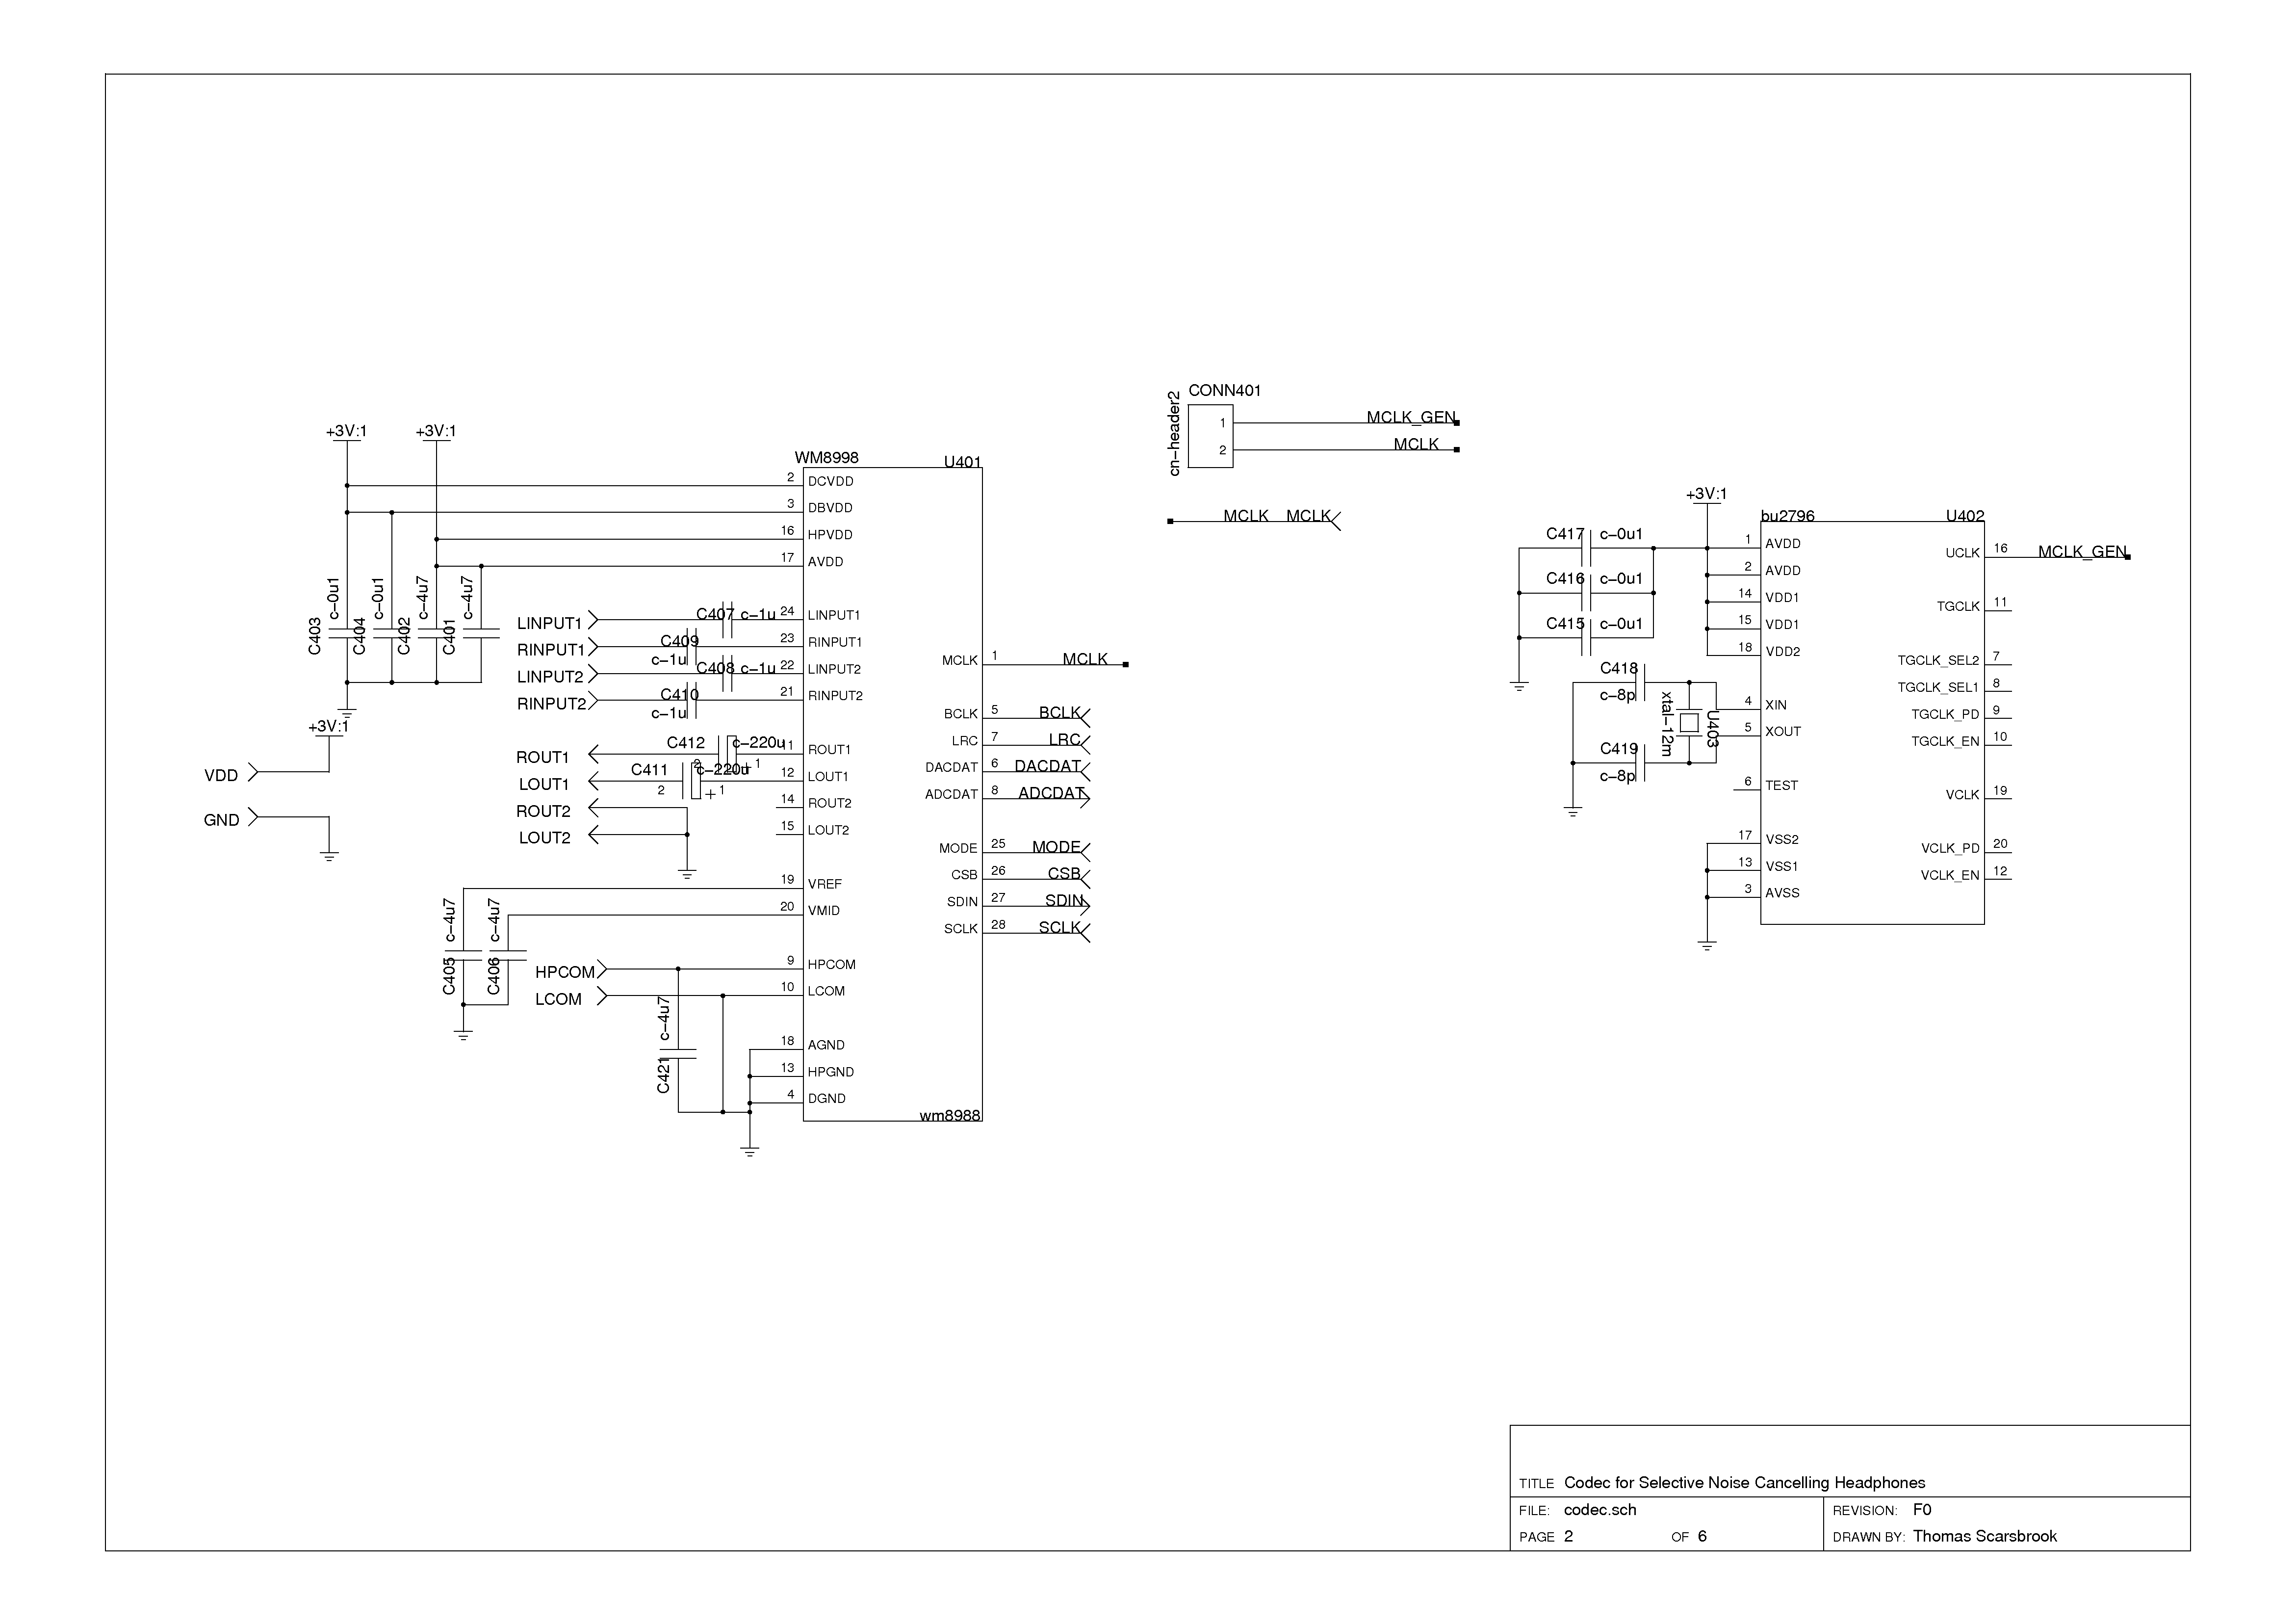
\includegraphics[width=\textwidth]{./img/codec.png}
	\caption{The schematic for the codec}
	\label{fig:codecsch}
\end{figure}

\subsubsection{Analogue}
Before the codec the signal needs some conditioning.
If any signal received were to be passed into the codec it could contain components at too high a frequency; these need to be removed to prevent aliasing.

\begin{figure}[H]
	\centering
	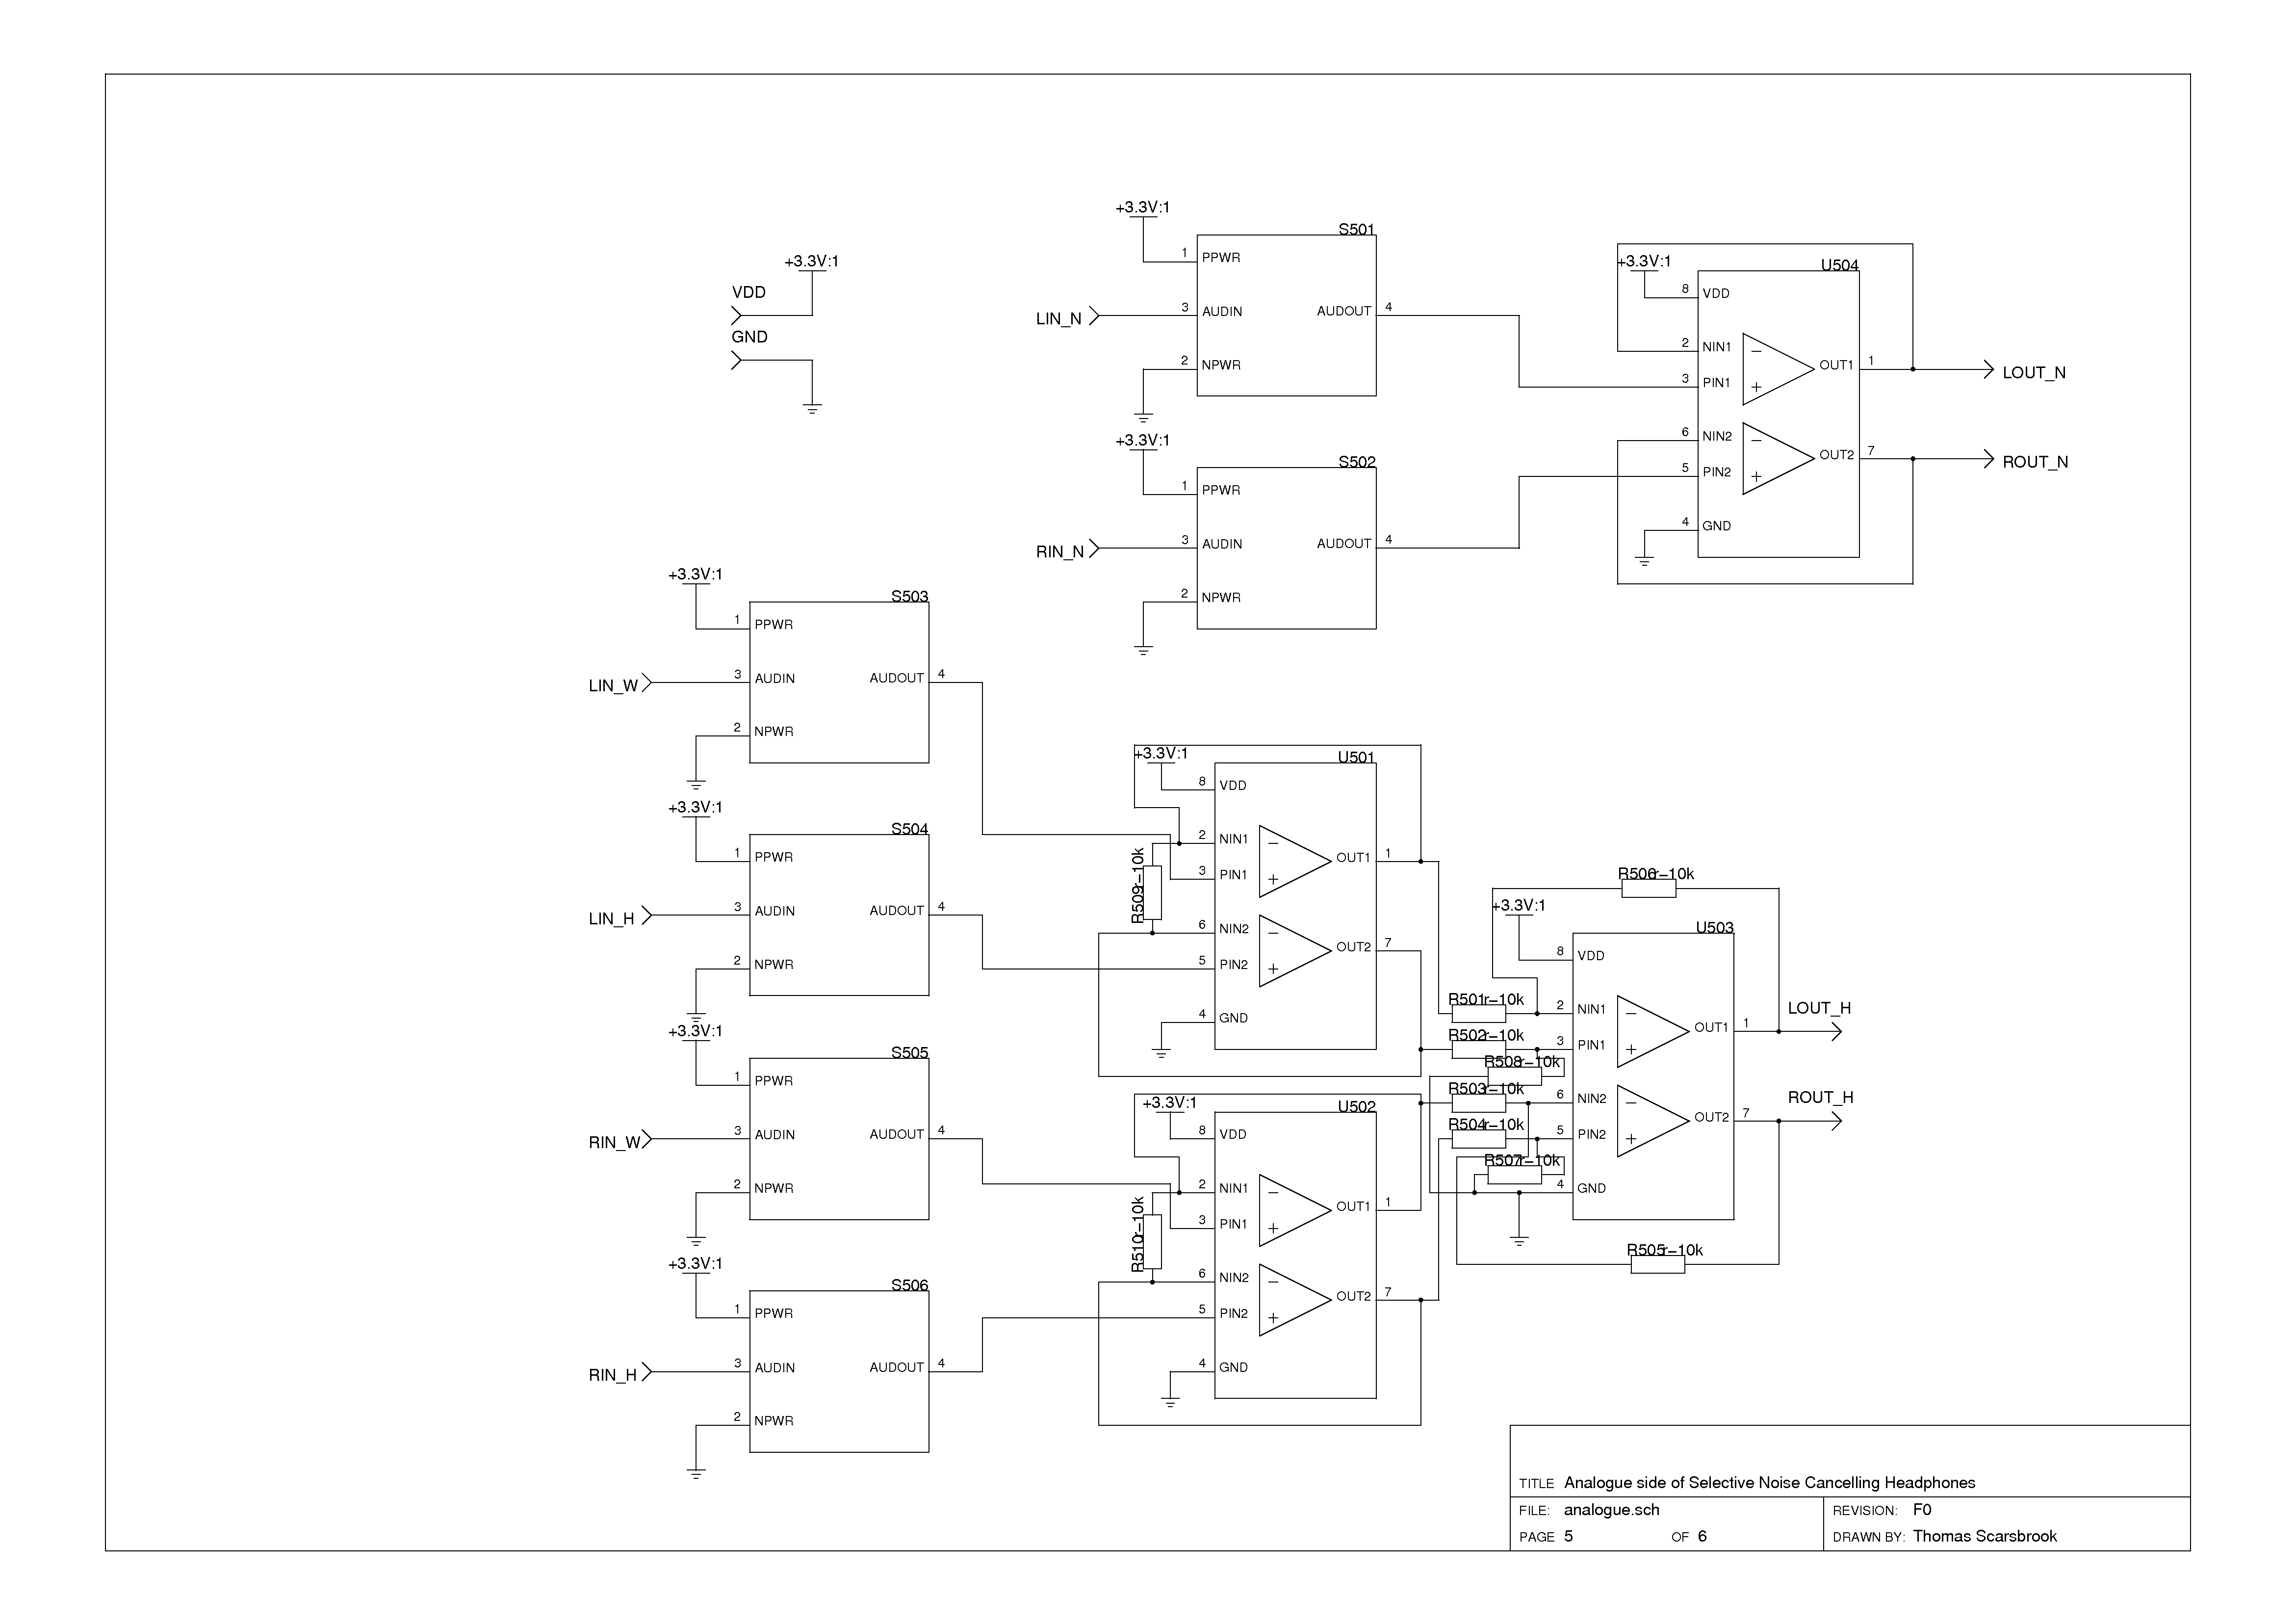
\includegraphics[width=\textwidth]{./img/analogue.png}
	\caption{The schematic of the analogue portion of the project}
	\label{fig:analoguesch}
\end{figure}

\noindent This portion of the design is then further split into two parts; the instrumentation amplifier, and the signal conditioning.
The instrumentation amplifier takes in the noise and the optional demanded signal, and sums the two together.
This choice of amplifier was based on a few requirements.
The inputs from the microphones on the headphones require the amplifier to have a large input impedance.
Using a naive summing amplifier would result in a much lower input impedance due to the mixing resistors.
In contrast, the demanded input is likely to be from an MP3 player or similar, which will provide a low output impedance due to being designed to connect direct to, and drive headphones.
As such this input does not require the same high impedance from the amplifier, however the signal is not harmed by it.
Providing this high impedance also allows microphones to be connected and still serve equally well.
The second requirement of the amplifier is that it must sum the signals together with minimal distortion to the heard signal.
Adding distortion would result in sub-optimal cancellation, due to the actual heard signal not being known.
The instrumentation amplifier is a difference amplifier, as such one of its inputs is affected by a phase shift of 180$^{\circ}$.
As the demanded signal has no specific requirement for phase being maintained, this signal is the one that gets inverted.
\\
\\
Signal conditioning is required in order to prevent aliasing occurring when the input signals are sampled.
In order to accomplish this a naive low-pass filter was used, as shown in figure \ref{fig:sigcondsch}.
This design was chosen due to its simplicity to implement and minimal power draw, whilst still maintaining a high input impedance and suitable roll-off.

\begin{figure}[H]
	\centering
	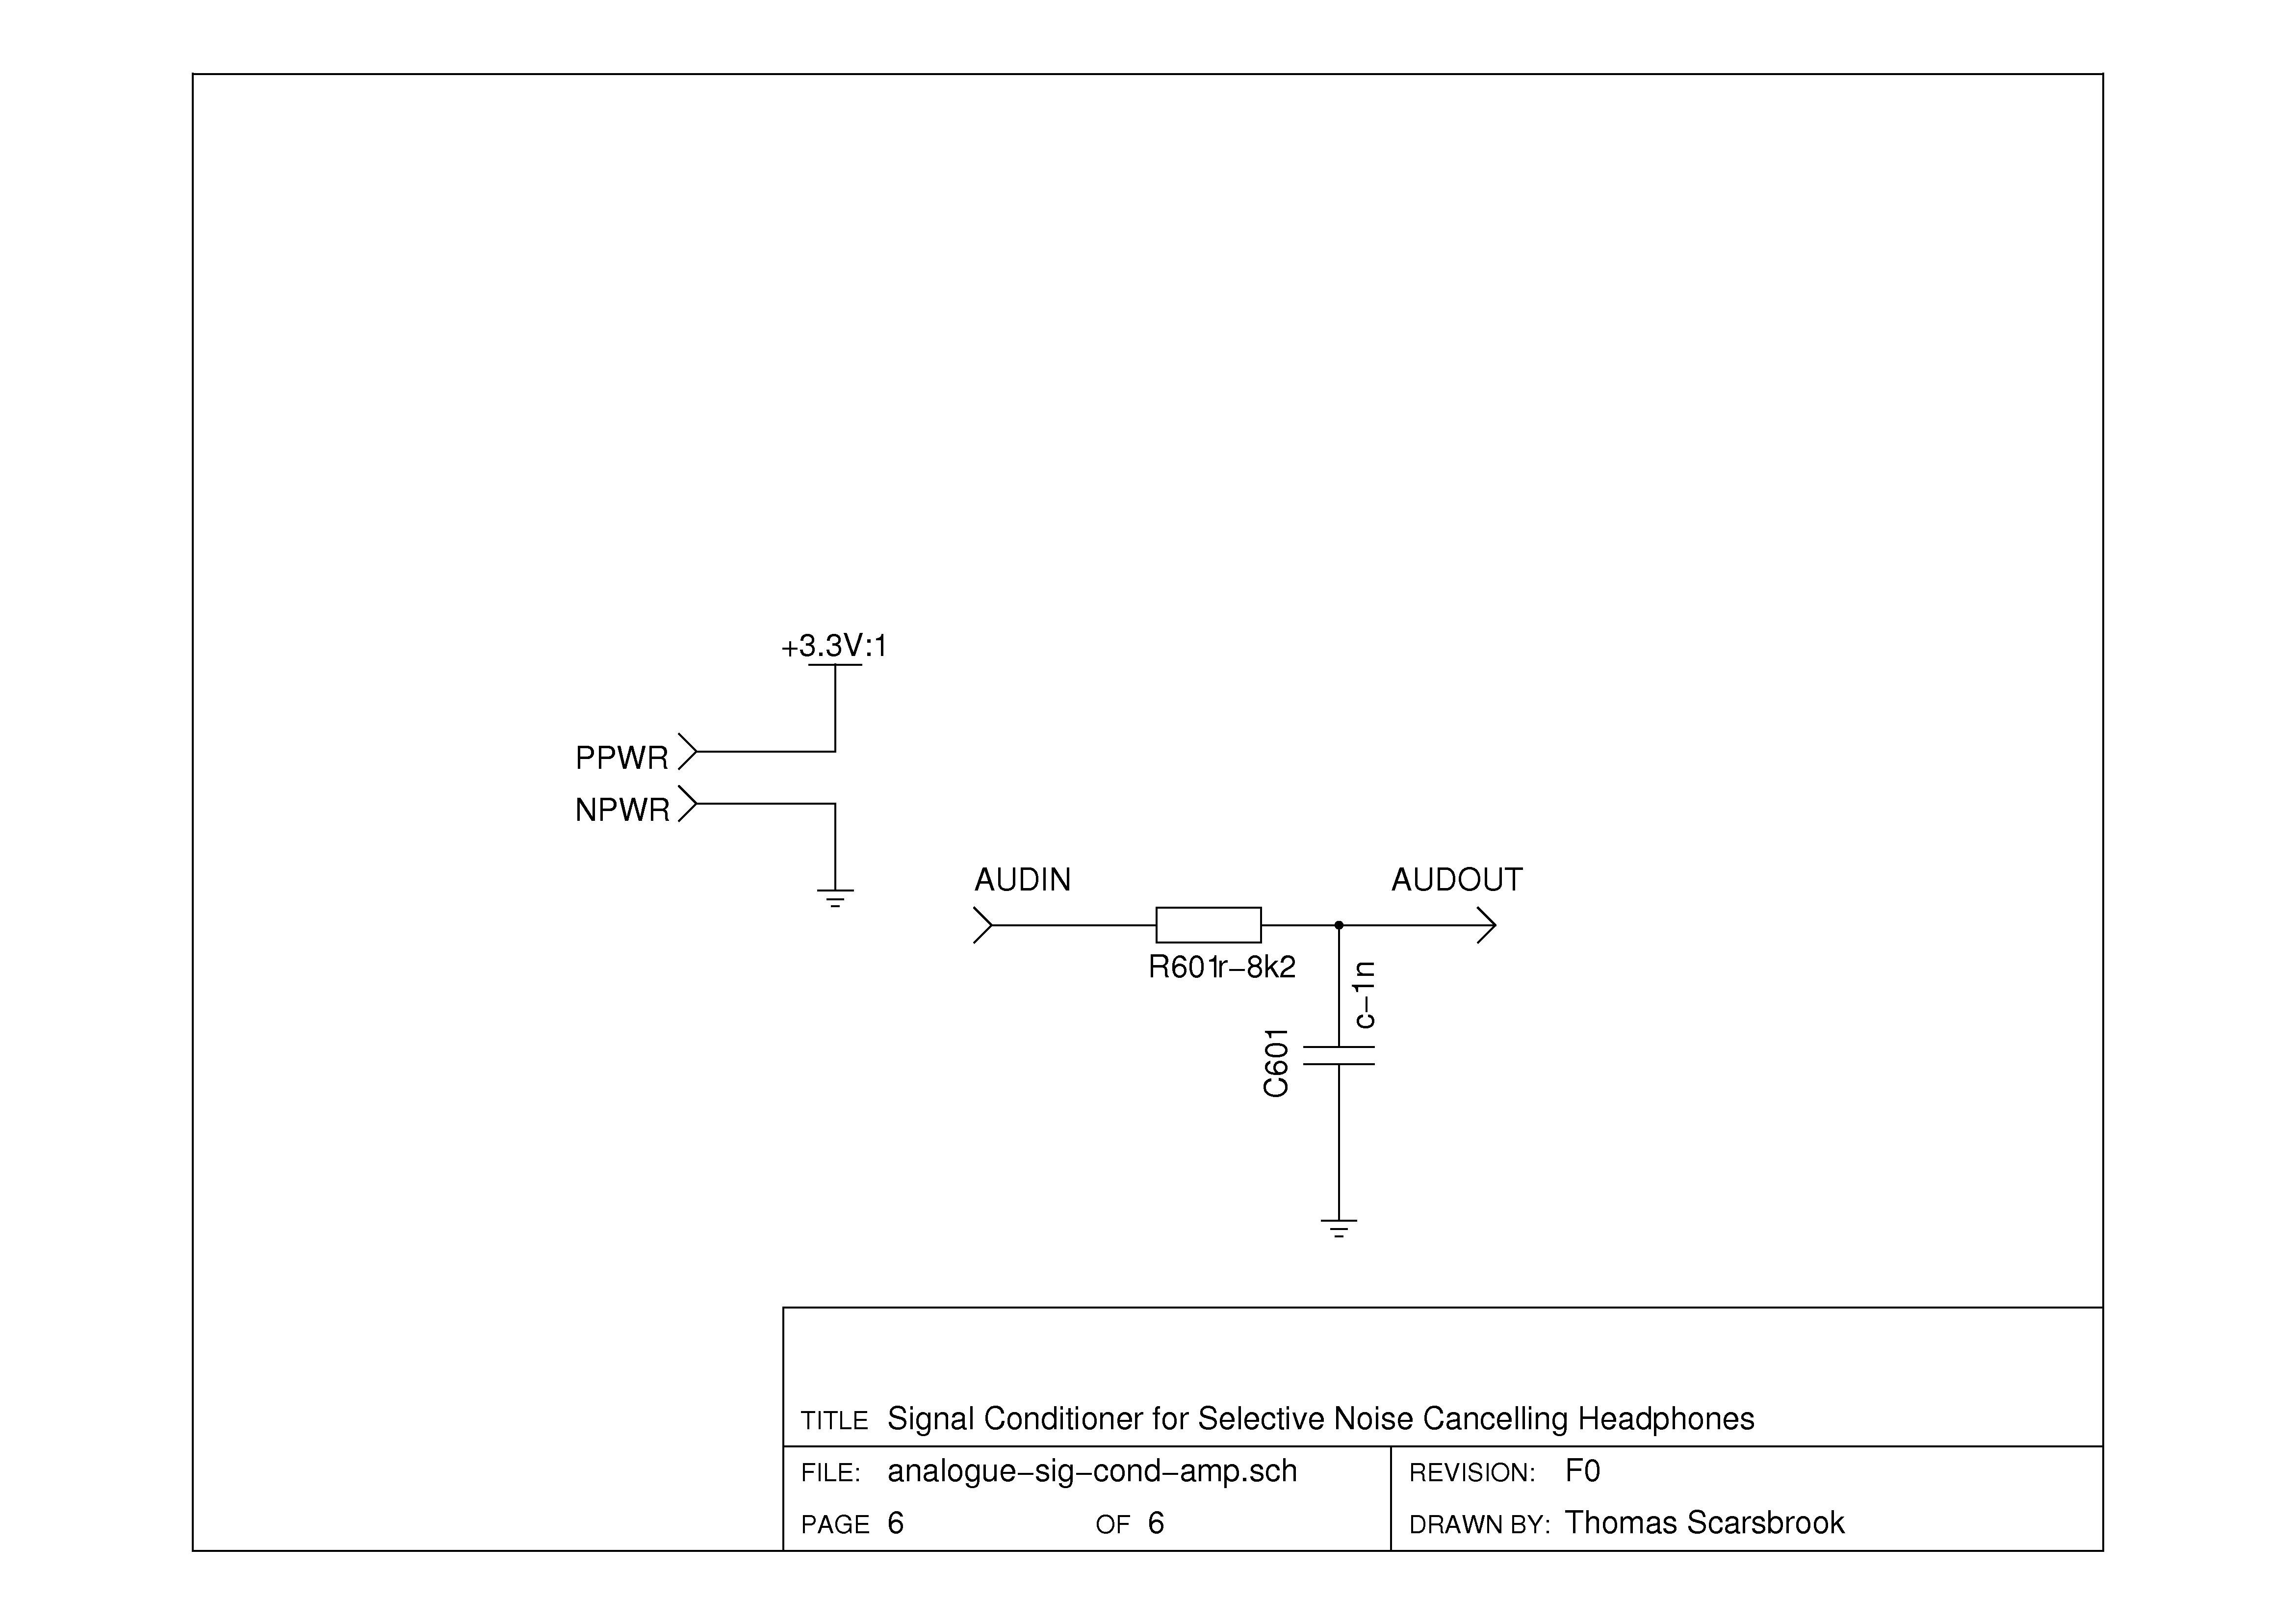
\includegraphics[width=\textwidth]{./img/analogue-sig-cond-amp.png}
	\caption{The signal conditioning amplifier schematic}
	\label{fig:sigcondsch}
\end{figure}

\noindent This design was tested through the use of a signal generator and digital oscilloscope.
The results can be seen below.

\subsubsection{Power}
One key part of any electronic system is it needs some form of power supply, and this project is no exception.
Multiple voltage rails were required, due to the DSP requiring a core voltage level as well as a second level for I/O.
The voltage level required by the codec and the amplifiers was the same as the one required by the DSP I/O, simplifying the design.

\begin{figure}[H]
	\centering
	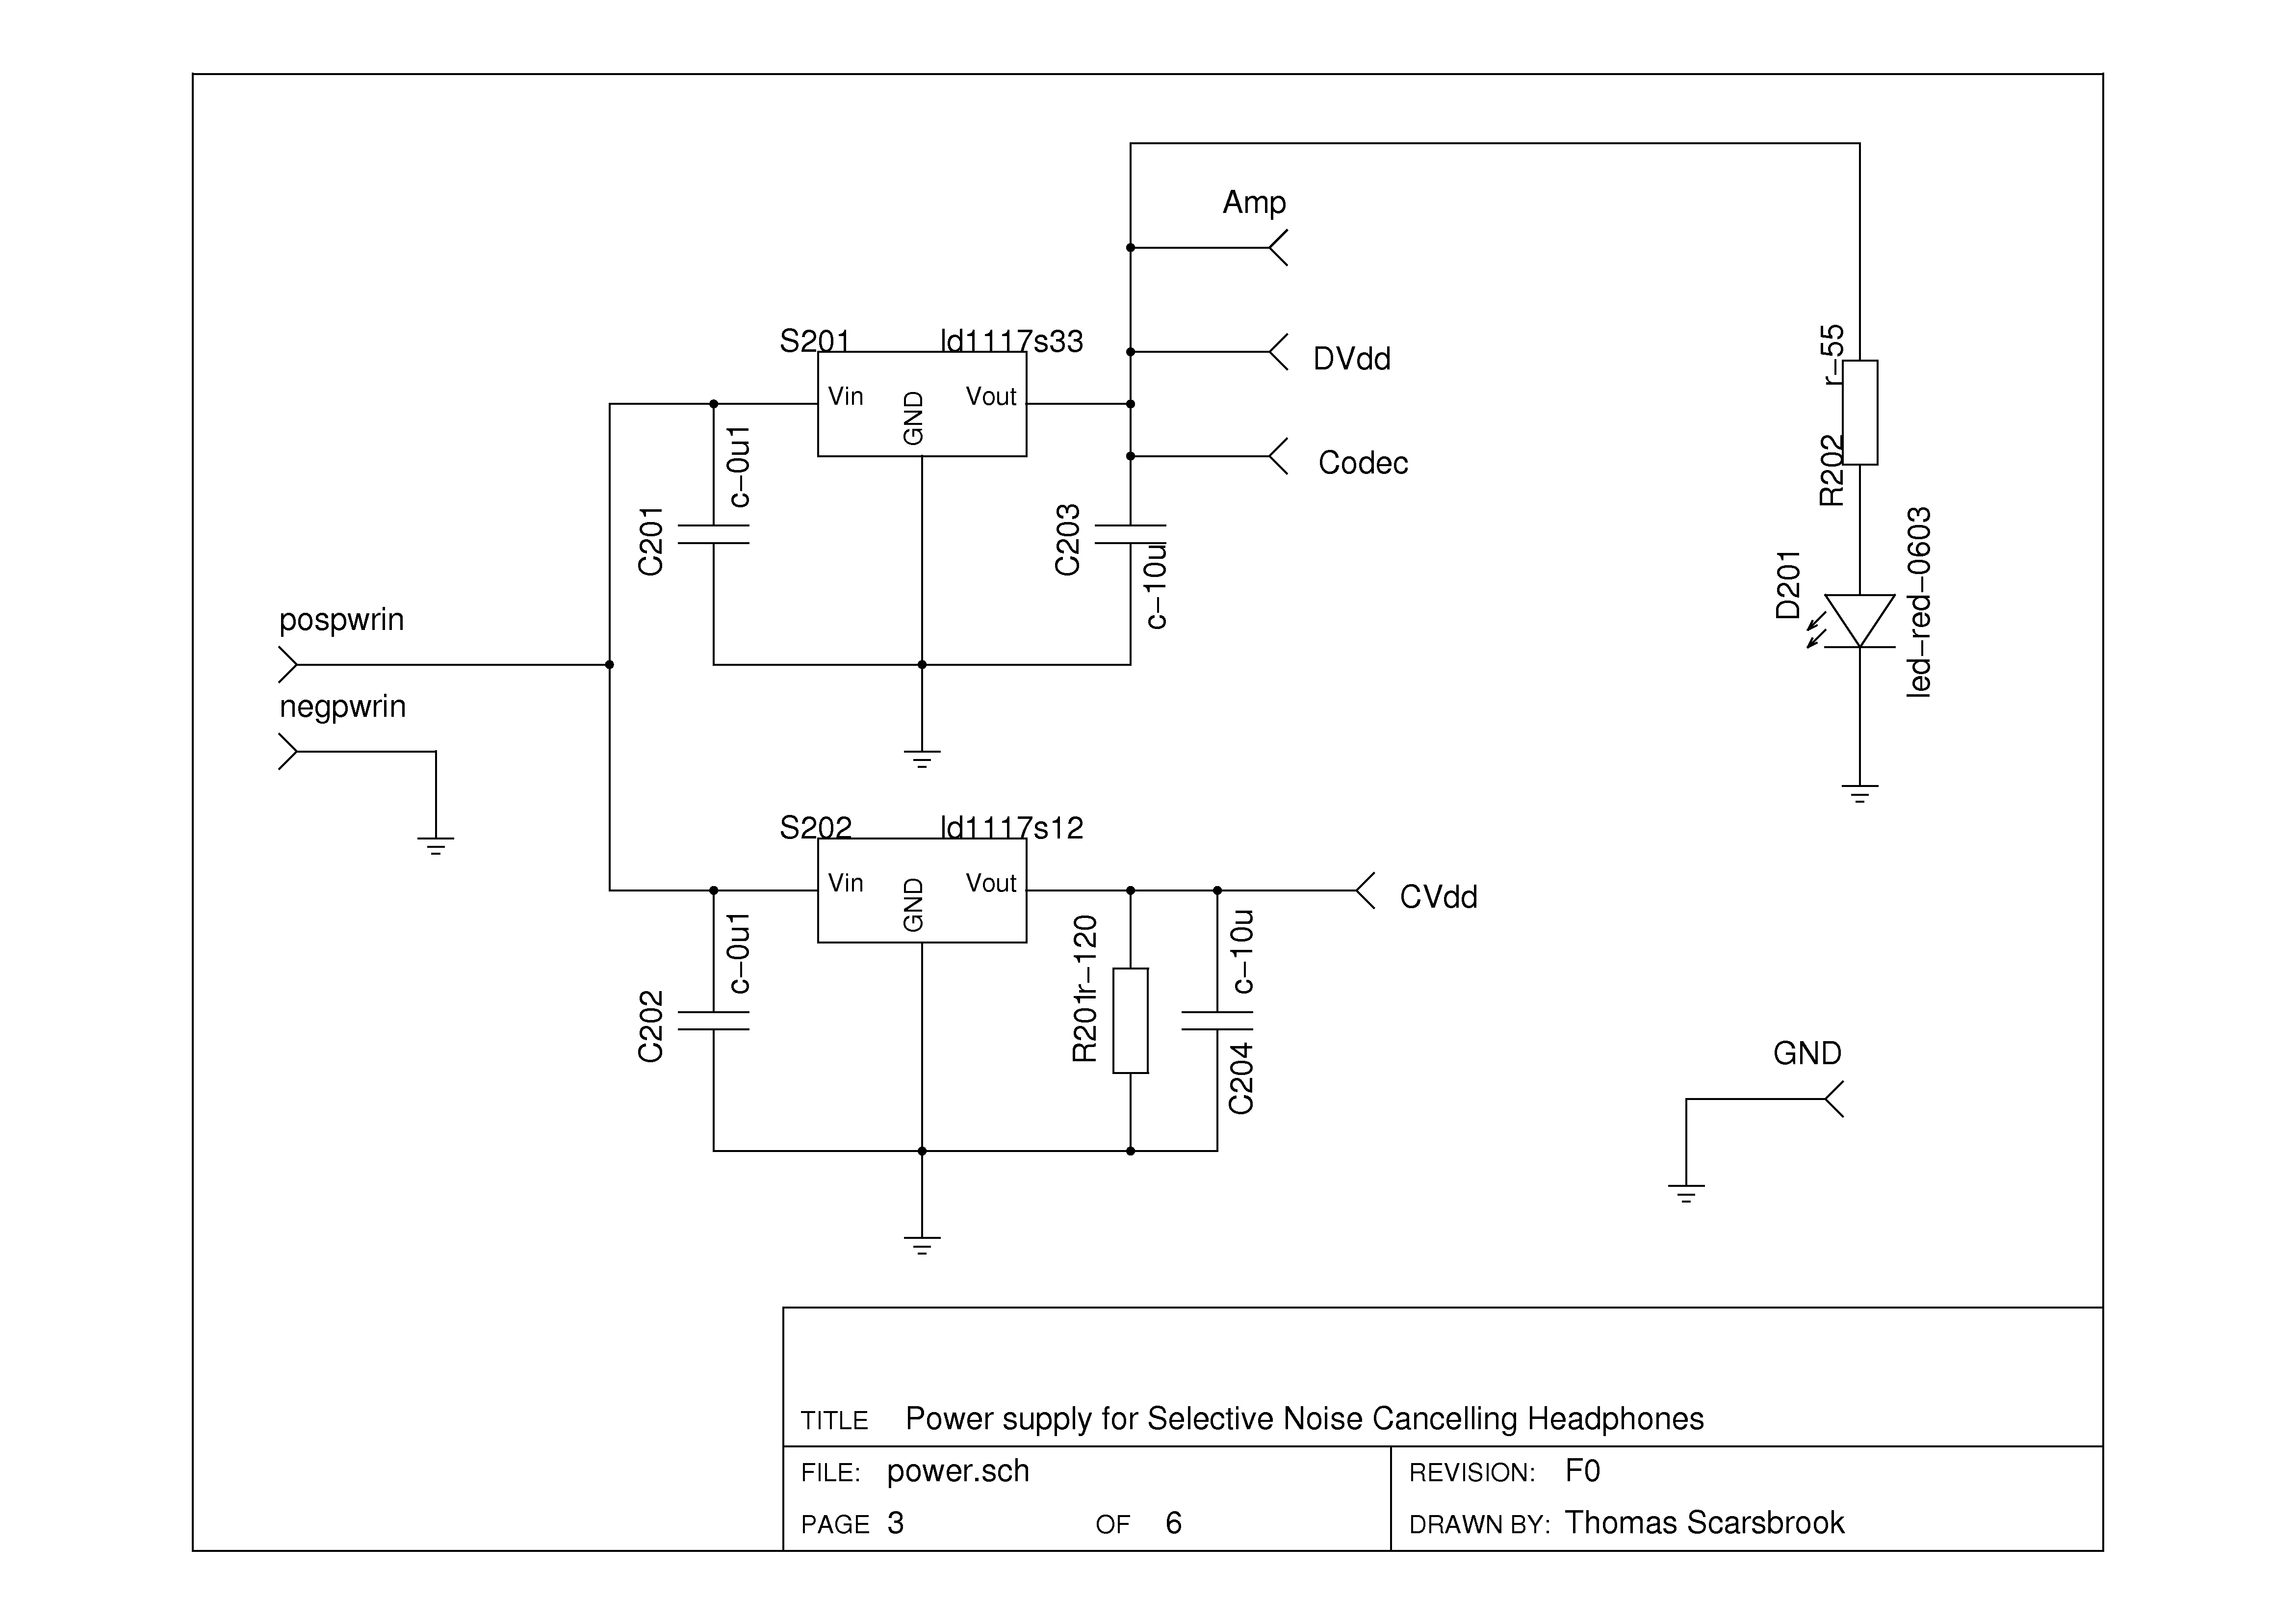
\includegraphics[width=\textwidth]{./img/power.png}
	\caption{The schematic of the power regulation for the projects PCB}
	\label{fig:powersch}
\end{figure}

\noindent In order to account for this two voltage regulators were obtained, one providing the 3.3V required by the DSP I/O and other circuitry, and the other providing the 1.2V required by the DSP core.
Both of these regulators were capable of providing 1.2A, which is in excess of the current requirements of the devices.
An LED was connected to the 3.3V rail to show when power was being provided, regardless of state of the rest of the system.

\begin{table}[H]
	\centering
	\begin{tabular}[c]{| l | c |}
		\hline
		\multicolumn{2}{|l|}{3.3V rail}\\
		\hline
		Component	& Draw (mA)	\\
		\hline
		DSP I/O		& 75	\\
		Codec		& 35.1	\\
		Clock Generator	& 160.6	\\
		Amplifiers	& 2	\\
		\hline
		Total		& 272.7	\\
		\hline
		\hline
		\multicolumn{2}{|l|}{1.2V rail}\\
		\hline
		Component	& Draw (mA)	\\
		\hline
		DSP core	& 625	\\
		\hline
		Total		& 625	\\
		\hline
	\end{tabular}	
	\caption{The current requirements of the various components in the circuits}
	\label{tab:pcbcurrentdraw}
\end{table}

\subsection{PCB}
Various things had to be taken into consideration for the PCB design.
The PCB was designed in gEDA PCB, due to previous experience with this software.

\subsubsection{Coupling}
For starters the high frequency switching involved in the digital portion of the system could introduce a lot of noise which could distort the signal from the analogue portion.
This would largely be seen as current being drawn along the ground plane, introducing a rapidly changing voltage gradient across it.
While this isn't as much of an issue for the digital portion, as there are margins around each voltage level, the analogue portion would suffer significantly, especially if the noise is introduced after the signal conditioning stage.
In order to mitigate this, the analogue circuitry has a separate ground plane to the digital.
Obviously these two ground planes still need to be connected to the same external connection, so they connect at this point, meaning minimal chance of currents flowing through the other portion of the system.
These separate planes can be seen in figures \ref{fig:pcbtop} and \ref{fig:pcbbottom}.
The digital ground planes are the red and light green planes respectively, whilst the analogue grounds are grey and dark green.
\\
\\
In order to place the analogue circuitry on its own ground plane, it had to be segregated from the rest of the circuitry.
This style was maintained with the rest of the layout, where circuits with different functions were kept separated from the rest.
Power kept separate from the DSP, the DSP kept separate from the codec, etc.
An additional benefit arose from this, where signals travelling between parts of the system were travelling a short distance reducing the effect of noise.
An example of this is the clock generator feeding the codec.
The 12MHz signal it provides would generate a large amount of noise, however as it is kept in a segment with the codec IC itself the signal has a very short distance to travel.
As such this signal did not interfere with other signals as there was no need for it to pass near them.
Also there was a portion of ground plane between it and other signals, preventing it from passing over.
\\
\\
Another way to help mitigate the noise effects is to place decoupling capacitors across the power rails near each IC.
This is something that is required with the digital systems as well as the analogue circuitry, as they are still susceptible to this noise effect albeit less so than the analogue.
Some of these decoupling capacitors can be seen around the codec and clock generator, however the more obvious ones are those around the DSP.
Due to its size and complexity the DSP requires more decoupling than the rest of the circuitry.
Multiple sizes of capacitors were used around the DSP.
In opposing corners of the DSP a 10$\mu$F capacitor was placed to remove lower frequency components and to give a reasonable power storage against drops.
Then around the edge of the DSP, right next to the pins that required them, smaller 1$\mu$F capacitors were placed to remove high frequency components right at the power entry.


\subsubsection{Layers and Packaging}
There are various different packages available for the components to be used on the PCB, and which packages are used affect the construction of the PCB.
The first, basic decision to be made was whether to use surface mount components, or through hole components.
Due to the low power nature of this system this choice was remarkably simple.
Using through hole components would require more physical space above and below the PCB surface than surface mount components, and would be more bulky width ways.
Also the location of the pin holes would have taken more space than the surface mount pads, as they require space on both sides of the PCB.
Finally some components are limited in what packages they are available in.
For example the DSP was only available in surface mount packages.
As such there was no benefit to using through hole components, therefore surface mount ones were chosen.
\\
\\
The DSP was only available in two varieties of packaging, Quad Flat Package (QFP) or Ball Grid Array (BGA).
These packagings had an effect on not only the footprint required, but also pin availability and the speed the DSP could run at.
BGA had 272 pads arranged in a ring, 4 pads wide, around the underneath edge of the IC.
In order to connect to all these pads multiple levels were required, most likely requiring power and ground to be carried on separate layers on the PCB.
Increasing the PCB to 4 layers to allow for this would drastically increase the cost of the PCB, ~\pounds180 rather than the ~\pounds80 paid.
Routing the connections in between the pads and locating the decoupling capacitors would have been rather difficult.
Also there is then an issue in terms of production.
A BGA package requires soldering onto the board in an oven.
On the plus side, in this package the DSP was available in speeds up to 300MHz.
\\
\\
On the other hand QFP has all the pins located across the four sides of the IC, and therefore only provides 208 pins due to the reduced area to connect with.
However all the pins of the package could be physically accessed externally, meaning that routing around them becomes much easier, also only a single layer is required to mount the device.
Soldering the package to the board becomes an easier task too, and a standard soldering iron can be used.
QFP loses out on the speed side though, the only speed available in a QFP package is 200MHz.
\\
\\
Taking these into account it was decided to use the QFP package in this project.
While fewer pins are available to the user, none of the pins that became unavailable were required by this project, as such the loss of them was not an issue.
The slower speed was a greater factor, however it was outweighed by the cost of manufacture that the BGA would have required, and testability.
Due to the fact that all the pins of the QFP package were physically accessible by the user, testing would be easier as they can be probed, whereas the BGA package does not allow this.
\\
\\
In order to reduce the size of the board required, to ease routing, and aid the placement of decoupling capacitors near the power connections, a two layer PCB was used.
This second layer allowed the decoupling capacitors to be placed directly beneath the pins they would connect to, reducing the distance from the pins and therefore reducing the amount of noise that could appear on the line.
However the more significant advantage was the ability for tracks that would otherwise conflict pass over each other.

\subsubsection{Debugging Headers}
Due to the fact this system was under development, the PCB would require vigorous testing after production.
In order to aid this testing a number of headers were placed between sections of the system, thus allowing the sections to be tested in isolation.
Not only could the output of a system be measured without the following stage affecting it, but also the input could be assigned manually without the preceding stage interfering.
Key placements of these headers were between the power and any other portion of the system, between the audio connections and the rest of the system, and on the interface between the analogue and digital portions of the system.


\begin{figure}[H]
	\centering
	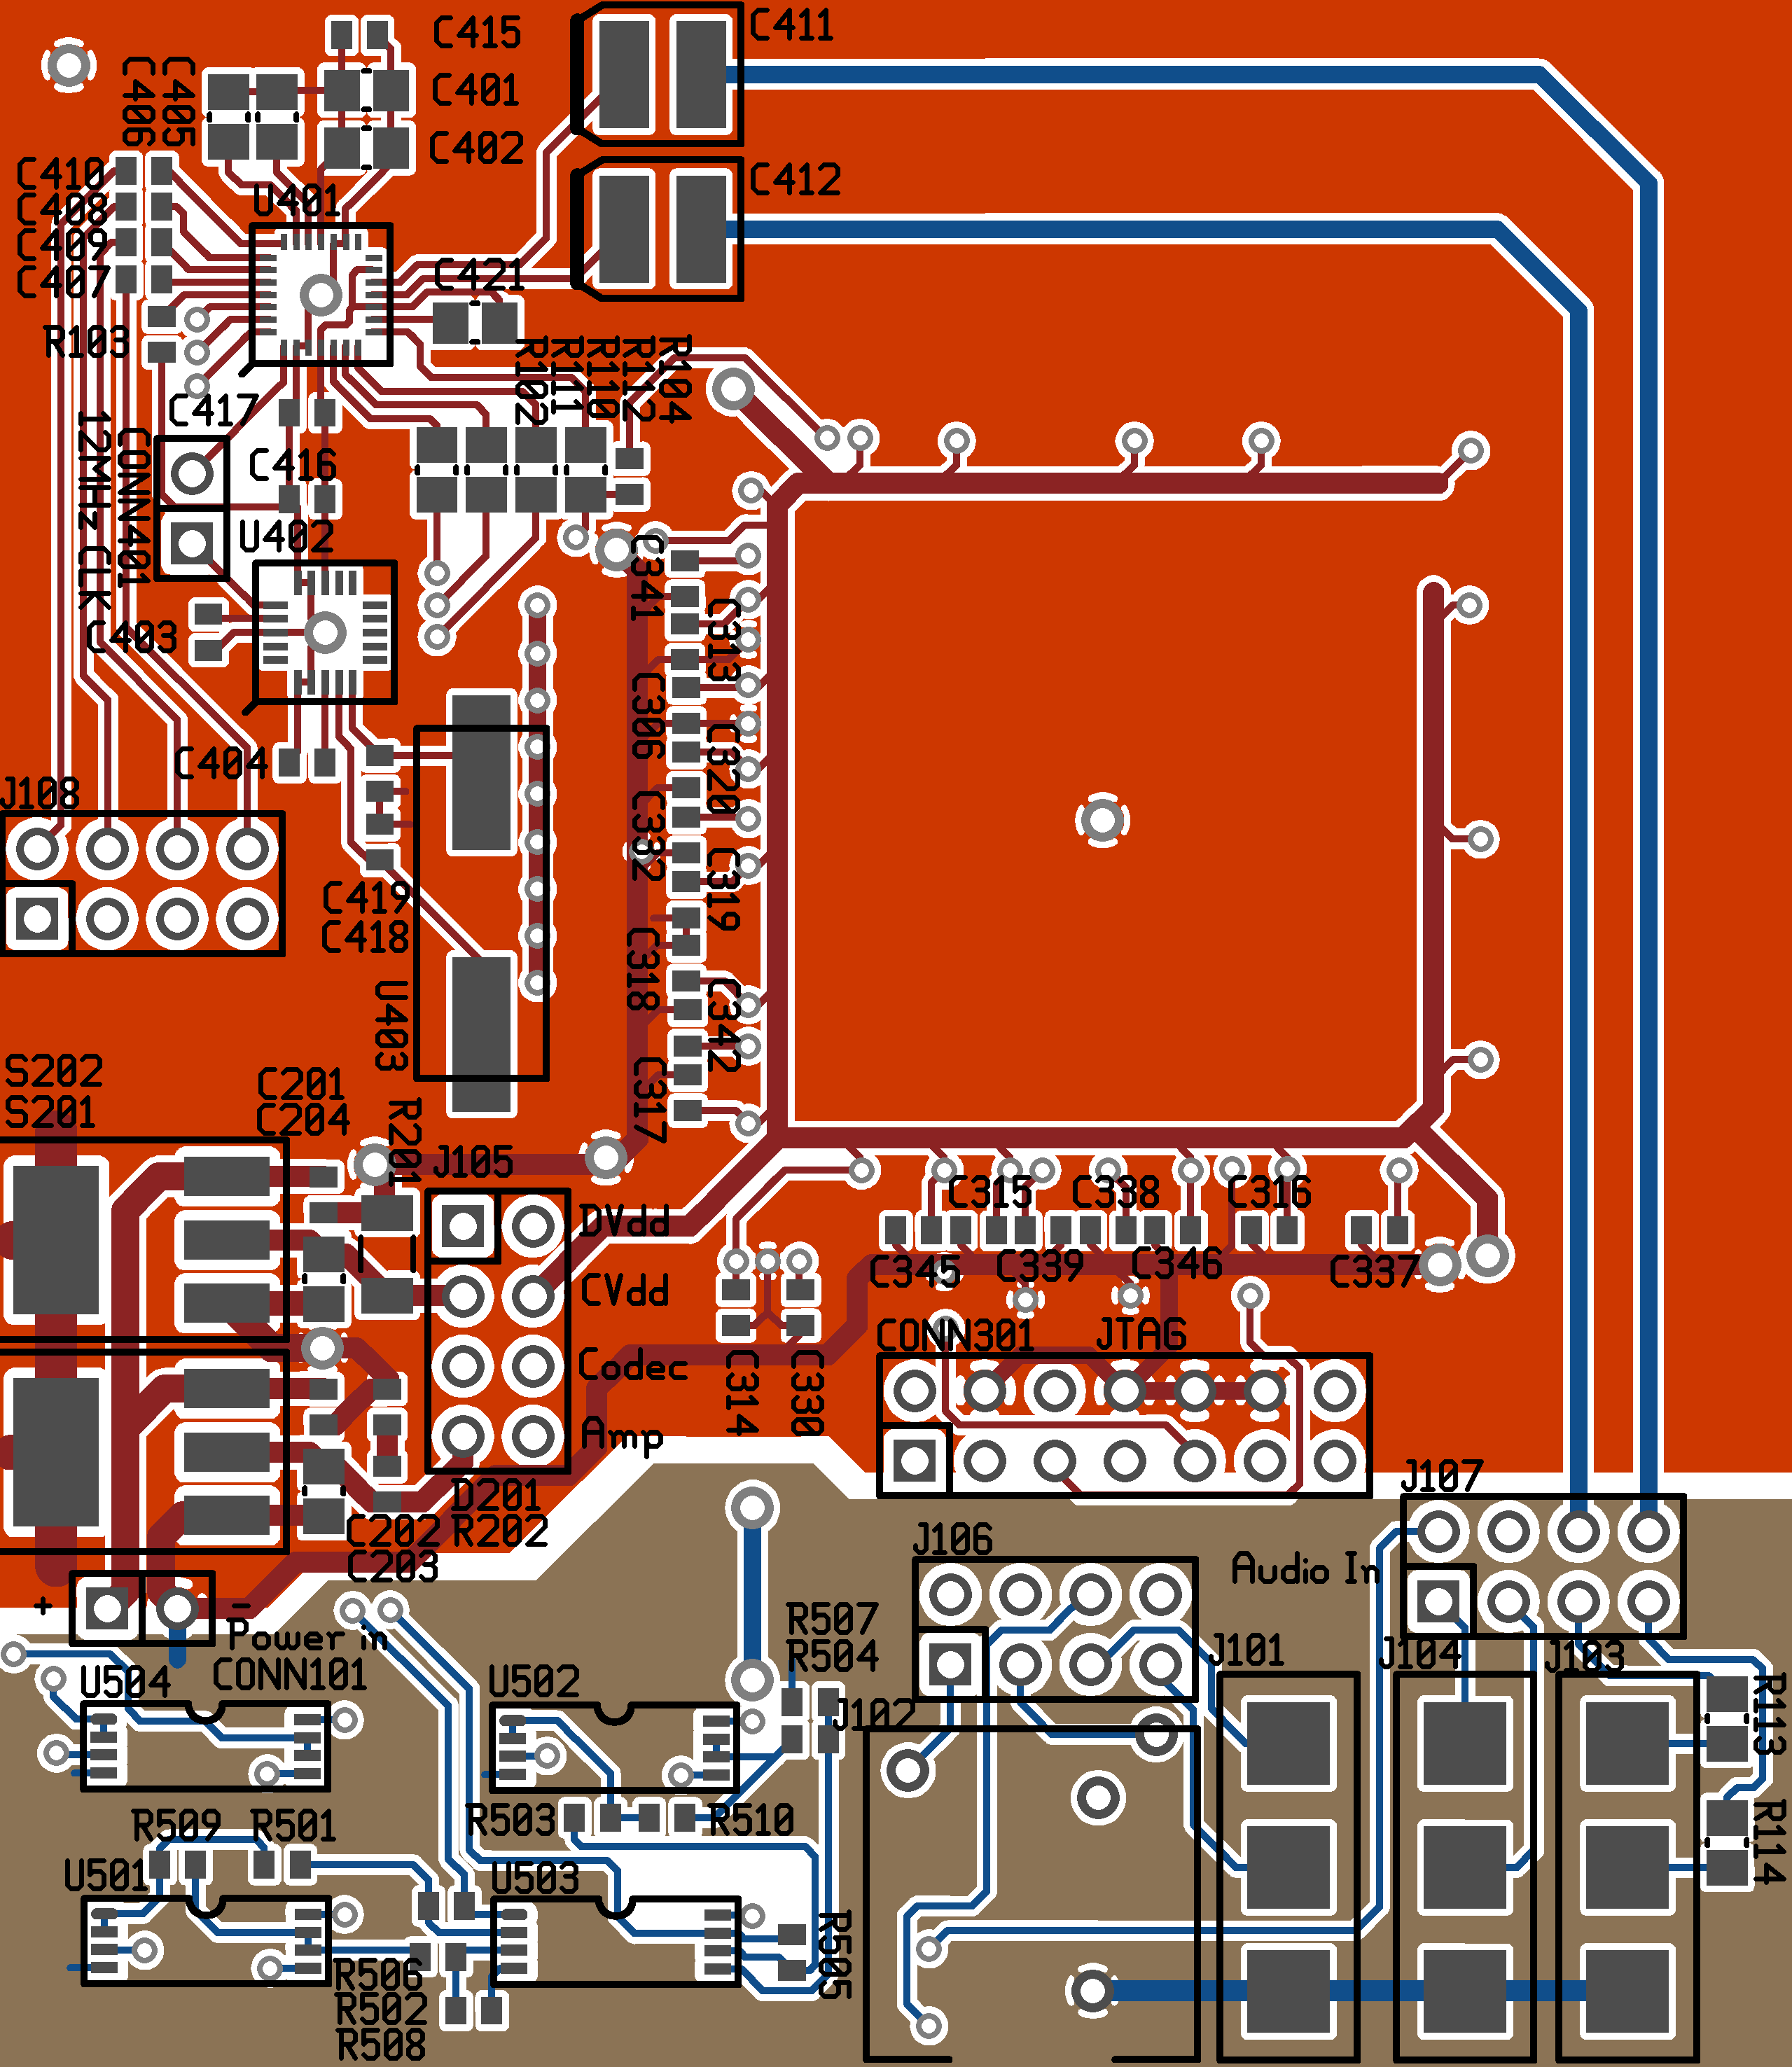
\includegraphics[width=280px]{./img/overview_top.png}
	\caption{The top side of the PCB}
	\label{fig:pcbtop}
\end{figure}
\begin{figure}[H]
	\centering
	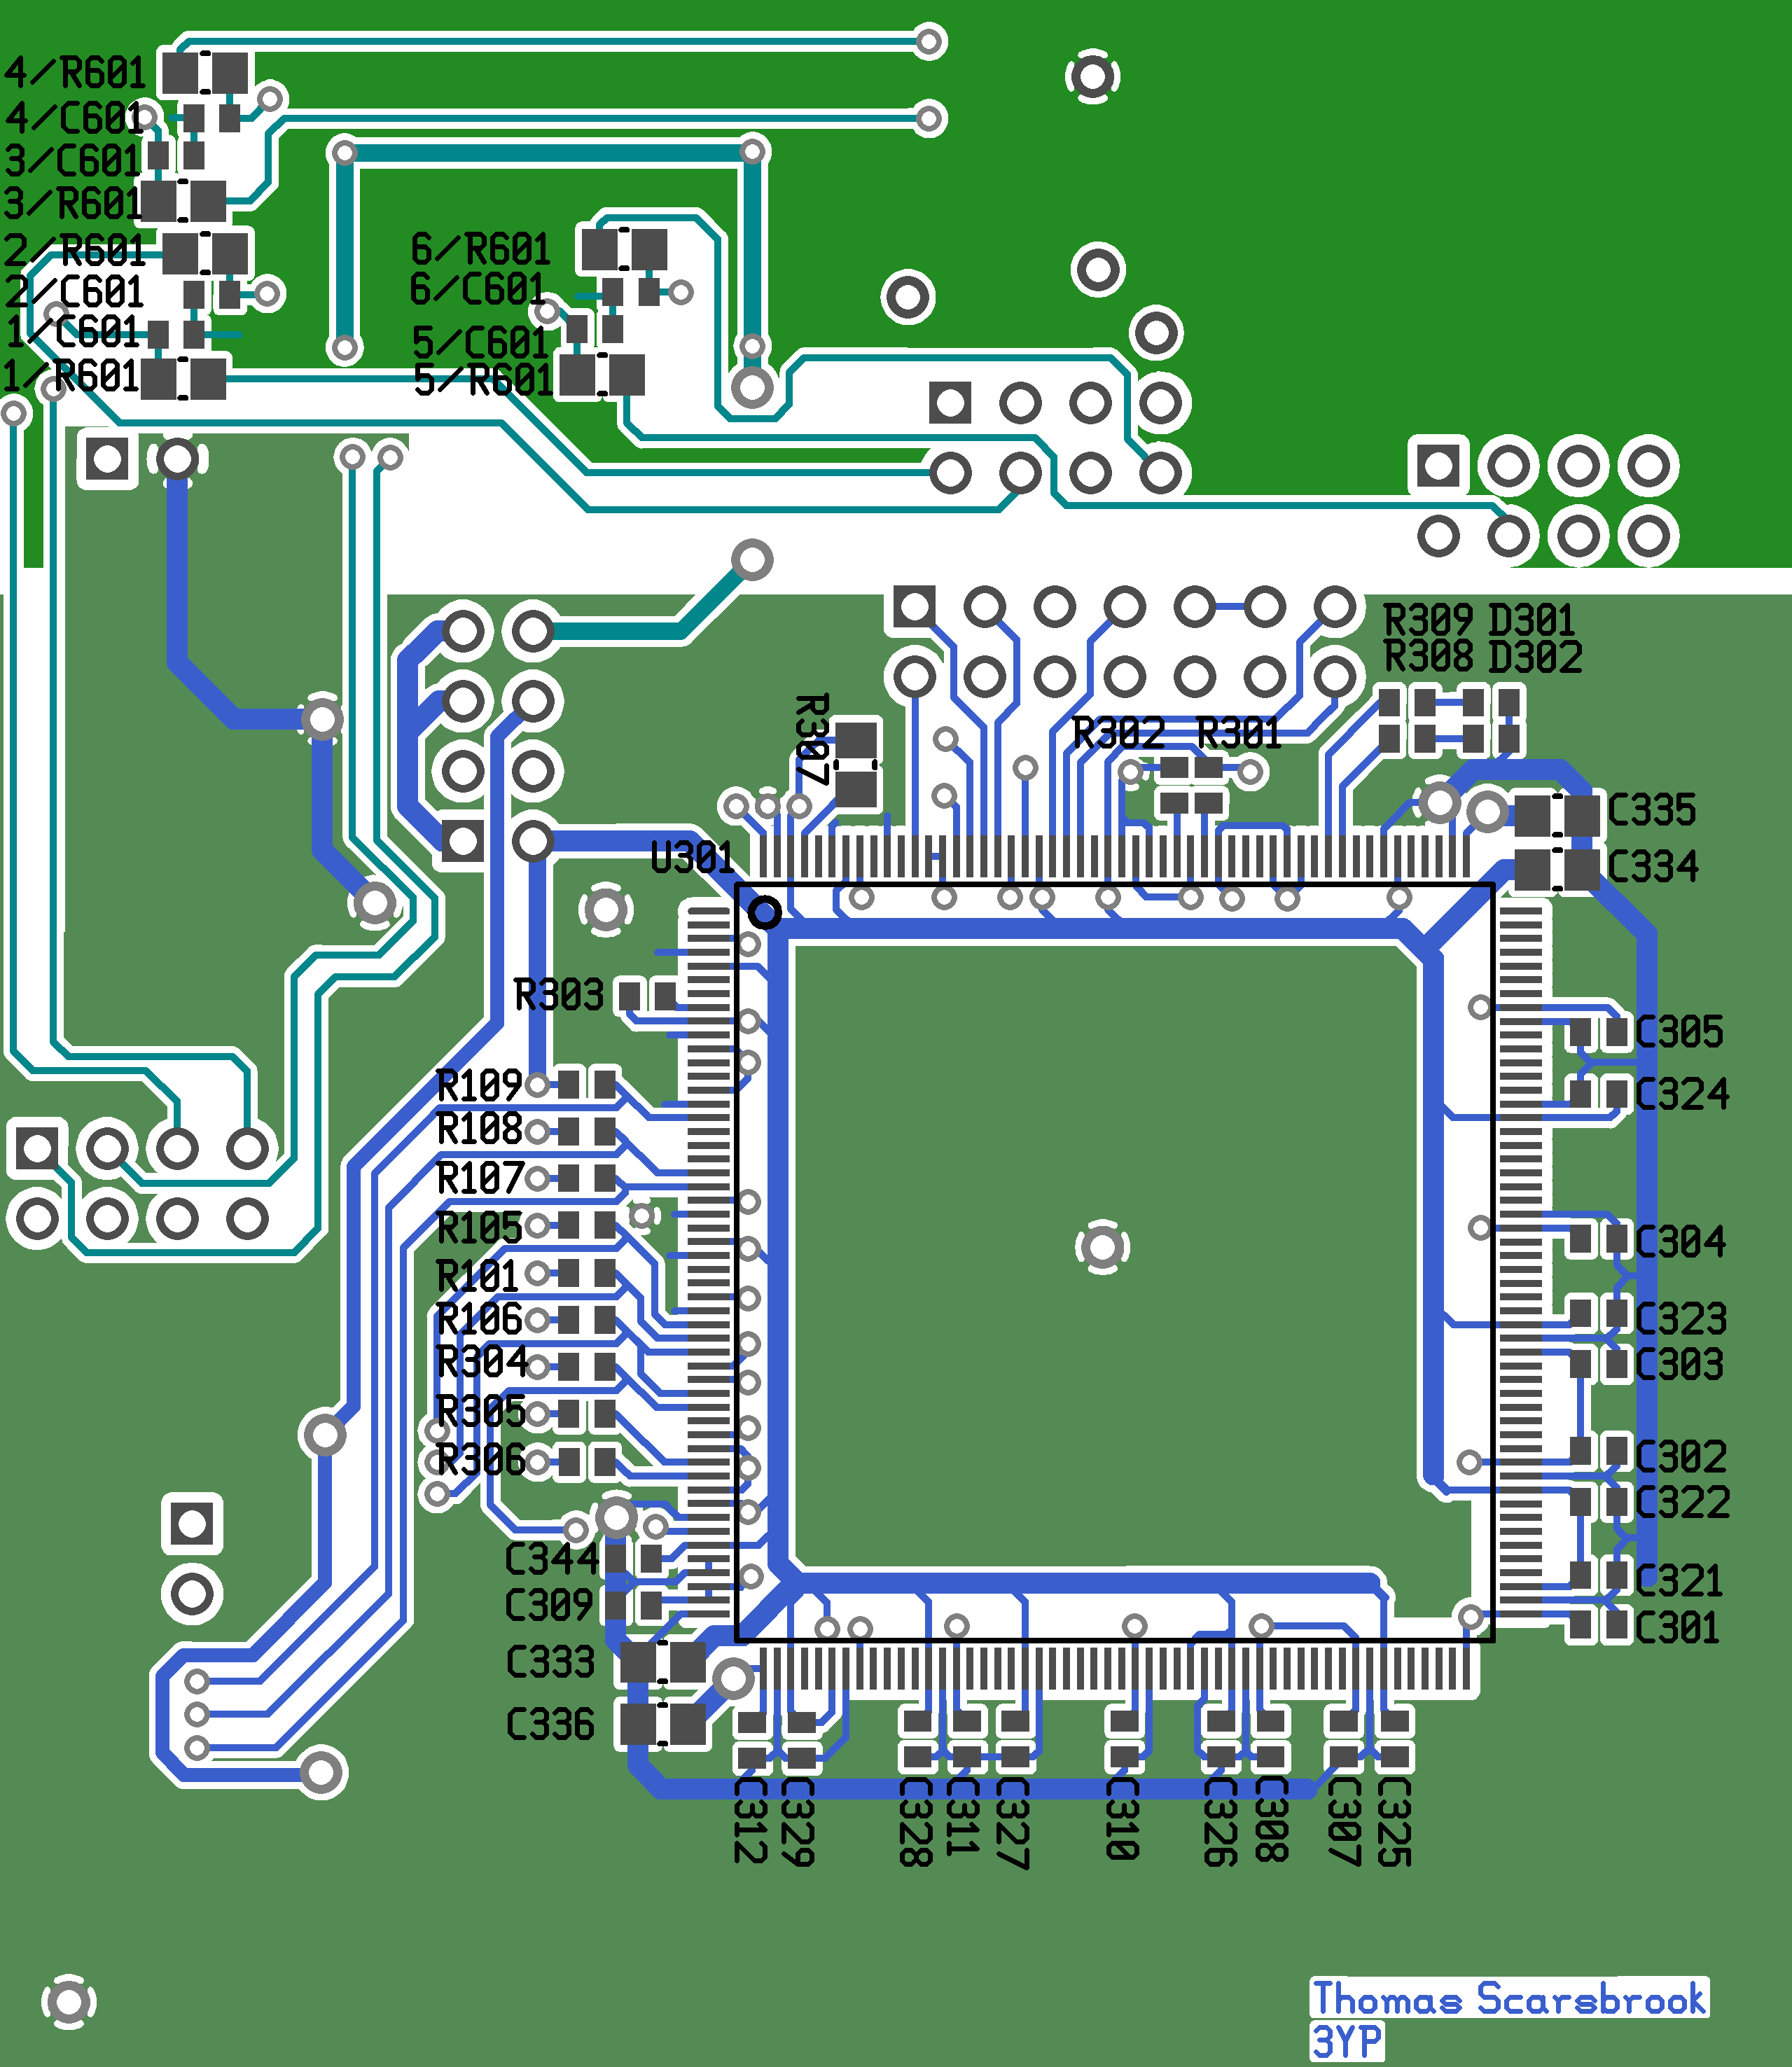
\includegraphics[width=280px]{./img/overview_bottom.png}
	\caption{The bottom side of the PCB}
	\label{fig:pcbbottom}
\end{figure}
